%%----------------------------------------------------------------------------------------
%	PACKAGES AND THEMES
%----------------------------------------------------------------------------------------
\PassOptionsToPackage{table}{xcolor}
\documentclass[aspectratio=169,xcolor=dvipsnames,svgnames,x11names,fleqn]{beamer}
% \documentclass[aspectratio=169,xcolor=dvipsnames,fleqn]{beamer}

\usetheme{RedVelvet}

\usefonttheme[onlymath]{serif}
\newcommand{\showanswers}{yes}
\usepackage{pifont} % For checkmarks and crosses

\usepackage{setspace}
\usepackage{xspace}
\usepackage{amsmath}
\usepackage{amssymb}
\usepackage{amsfonts}
\usepackage{color}
\usepackage{physics}
% \usepackage{mathbb}
\usepackage{rahul_math}
\usepackage{bigints}

\usepackage[utf8]{inputenc}
\usepackage[ruled,vlined]{algorithm2e}
\usepackage{amsmath}
\usepackage{amsfonts}

\usepackage{graphicx} % Allows including images
\usepackage{booktabs} % Allows the use of \toprule, \midrule and \bottomrule in tables
\usepackage{tikz,pgfplots}
\usepackage{mathtools}
\usepackage{subfigure}
\usetikzlibrary{arrows}
\usepackage{minted}
\definecolor{LightGray}{gray}{0.9}
\definecolor{cream}{rgb}{0.92, 0.9, 0.55}
\definecolor{lightblue}{rgb}{0.68, 0.85, 0.9}


\usepackage{xcolor-material}
\usetikzlibrary{fit}
\usetikzlibrary{matrix}
\tikzset{%
apple/.pic={
    \fill [MaterialBrown] (-1/8,0)  arc (180:120:1 and 3/2) coordinate [pos=3/5] (@)-- ++(1/6,-1/7)  arc (120:180:5/4 and 3/2) -- cycle;
    \fill [MaterialLightGreen500] (0,-9/10)  .. controls ++(180:1/8) and ++(  0:1/4) .. (-1/3,  -1) .. controls ++(180:1/3) and ++(270:1/2) .. (  -1,   0) .. controls ++( 90:1/3) and ++(180:1/3) .. (-1/2, 3/4) .. controls ++(  0:1/8) and ++(135:1/8) .. (   0, 4/7)
    }
    }

\newcommand{\leftdoublequote}{\textcolor{blue}{\scalebox{3}{``}}}

\newcommand{\rightdoublequote}{\textcolor{blue}{\scalebox{3}{''}}}


\usepackage{textcomp}
\usepackage{fontawesome}
\usepackage{tikz,pgfplots}
\usetikzlibrary{shapes.callouts}
\usetikzlibrary{arrows}
\usetikzlibrary{shapes.geometric, positioning}
\usetikzlibrary{matrix,positioning,decorations.pathreplacing,calc}
\usepackage{tikz-dependency}

\pgfplotsset{compat=1.8} % or newest version

\usetikzlibrary{positioning}


\usepackage{bm}
\usepackage{relsize}

\tcbuselibrary{skins, hooks}

\tikzset{basic/.style={draw,fill=MediumBlue!20,text width=1em,text badly centered}}
\tikzset{input/.style={basic,circle}}
\tikzset{weights/.style={basic,rectangle}}
\tikzset{functions/.style={basic,circle,fill=MediumBlue!10}}



\usepackage{listofitems} % for \readlist to create arrays
\tikzstyle{mynode}=[thick,draw=MediumBlue,fill=MediumBlue!20,circle,minimum size=22]


\usepackage{overpic}

%----------------------------------------------------------------------------------------
%	TITLE PAGE
%----------------------------------------------------------------------------------------

\usepackage{tikz-qtree,tikz-qtree-compat}
\usetikzlibrary{tikzmark}
\usetikzlibrary{calc}

\usetikzlibrary{fit}
\tikzset{%
apple/.pic={
    \fill [MaterialBrown] (-1/8,0)  arc (180:120:1 and 3/2) coordinate [pos=3/5] (@)-- ++(1/6,-1/7)  arc (120:180:5/4 and 3/2) -- cycle;
    \fill [MaterialLightGreen500] (0,-9/10)  .. controls ++(180:1/8) and ++(  0:1/4) .. (-1/3,  -1) .. controls ++(180:1/3) and ++(270:1/2) .. (  -1,   0) .. controls ++( 90:1/3) and ++(180:1/3) .. (-1/2, 3/4) .. controls ++(  0:1/8) and ++(135:1/8) .. (   0, 4/7)
}
}
\usepackage{tikz-qtree,tikz-qtree-compat}
\usetikzlibrary{tikzmark}
\usetikzlibrary{calc}

\usetikzlibrary{positioning}

% Define styles
\tikzset{
    box/.style={
        rectangle,
        draw=black,
        fill=blue!20,
        text width=2.2cm,
        text centered,
        minimum height=0.8cm,
        font=\small
    },
    arrow/.style={
        ->,
        >=Stealth,
        line width=1.5pt,
        draw=black
    }
}


\usepackage{bm}
\usepackage{relsize}



\tikzset{basic/.style={draw,fill=MediumBlue!20,text width=1em,text badly centered}}
\tikzset{input/.style={basic,circle}}
\tikzset{weights/.style={basic,rectangle}}
\tikzset{functions/.style={basic,circle,fill=MediumBlue!10}}
\usetikzlibrary{arrows.meta, bending}
\usetikzlibrary{shapes.geometric, arrows.meta, positioning, fit, backgrounds}

\usepackage{listofitems} % for \readlist to create arrays
\tikzstyle{mynode}=[thick,draw=MediumBlue,fill=MediumBlue!20,circle,minimum size=22]


\newmdenv[
backgroundcolor=androidYellowLight,
linecolor=androidYellow,
linewidth=0.5pt,
roundcorner=10pt,
skipabove=\baselineskip,
skipbelow=\baselineskip
]{MintedFrame}

% Set minted options
\setminted{
fontsize=\footnotesize,
breaklines=true,
autogobble,
linenos,
frame=none
}


\title[CPE 487/587: Deep Learning]{CPE 486/586: Deep Learning for Engineering Applications} % The short title appears at the bottom of every slide, the full title is only on the title page
\subtitle{07 Variational AutoEncoder}

\author[Rahul Bhadani] {{\Large \textbf{Rahul Bhadani}}}

\institute[UAH] % Your institution as it will appear on the bottom of every slide, maybe shorthand to save space
{
    Electrical \& Computer Engineering,  The University of Alabama in Huntsville
}
\date

% \titlegraphic{
%    \includegraphics[width=0.4\linewidth]{figures/UAH_primary.png}
% }

\begin{document}

%-------------------------------------------------
\begin{frame}
    \titlepage
\end{frame}

%-------------------------------------------------
\begin{frame}{Outline}
    \backgroundtableofcontents
\end{frame}

\section{Motivation}

\begin{frame}
    \sectionpage
\end{frame}

%\begin{frame}{Estimating Probability Pistribution for Generative Processes}
%
%\Large 
%
%\begin{center}
%Given $\xbf$, we want to estimate $P(\xbf)$ that gives a complete description of the probabilistic model that generates the observed data.
%
%\end{center}
%
%We want to learn generative processes to that can generate more dataset, at the same time, discard noise to truly learn physical laws. Generative processes can also provides ways to express causal relations.
%
%E.g. if we understand the generative process of wildfire, we can apply the knowledge to California or Australia.
%
%In this lecture, we model generative processes using Variational Autoencoder.
%\end{frame}

\begin{frame}{Estimating Probability Distributions for Generative Processes}
    
    % Main Objective Box
    \begin{tcolorbox}[colback=softblue, colframe=mainblue, arc=4pt, boxrule=1pt, left=10pt, right=10pt, top=8pt, bottom=8pt]
        \centering 
        Given $\mathbf{x}$, we aim to estimate $P(\mathbf{x})$ to provide a complete description of the probabilistic model that generates the observed data.
    \end{tcolorbox}

    \vspace{0.1cm}
\footnotesize

    \begin{itemize}
        \item \textbf{Data Synthesis:} We want to learn generative processes capable of producing new datasets.
        \item \textbf{Noise Reduction:} By discarding noise, we can more effectively learn underlying physical laws.
        \item \textbf{Causality:} Generative models provide a framework to express and understand causal relations.
    \end{itemize}

    \vspace{0.1cm}

    % Example with an accent
    \begin{tcolorbox}[blanker, borderline west={2pt}{0pt}{gray!40}, left=10pt]
        \small \textit{\textbf{Example:} If we understand the generative process of wildfires, we can apply that knowledge across different regions, such as California or Australia.}
    \end{tcolorbox}



    % TikZ Visualization of VAE/Generative Process
    \begin{center}
    \begin{tikzpicture}[node distance=7cm, font=\sffamily\small]
        \node (latent) [circle, draw=mainblue, thick, fill=softblue] {Latent Space};
        \node (output) [rectangle, draw=darkgray, thick, right of=latent, xshift=1.5cm, fill=gray!10] {$\hat{\mathbf{x}}$ (Generated Data)};
        
        \draw [-{Stealth[scale=1.2]}, thick, mainblue] (latent) -- node[above] {Generative Model} (output);
    \end{tikzpicture}
    \end{center}

    \centering
    \textbf{In this lecture, we model generative processes using Variational Autoencoders (VAEs).}

\end{frame}
    

    \section{AutoEncoder}

\begin{frame}
    \sectionpage
\end{frame}

\begin{frame}{What is AutoEncoder}

    \begin{columns}[T]
        \begin{column}{0.49\textwidth}
            \centering
\resizebox{0.8\textwidth}{!}
{
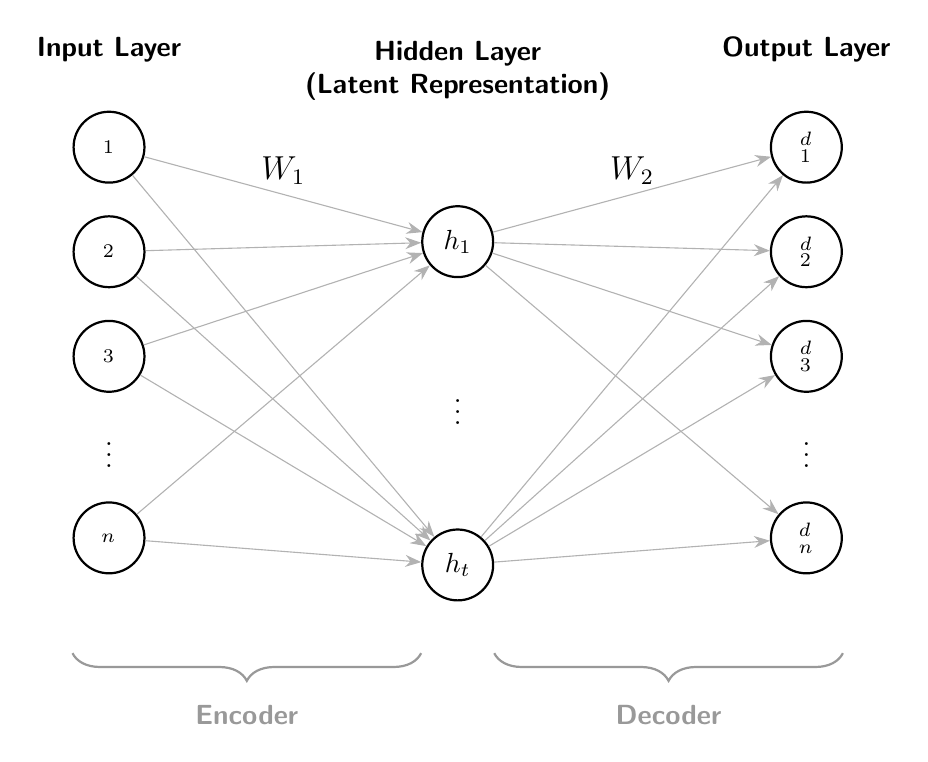
\begin{tikzpicture}[
    % Global Style Definitions
    node distance=1.2cm and 2.5cm,
    layer_node/.style={circle, draw=black, thick, minimum size=0.9cm, inner sep=0pt, fill=white, font=\sffamily},
    label_text/.style={font=\sffamily\bfseries, text centered},
    brace_style/.style={decorate, decoration={brace, amplitude=10pt, mirror}, thick, gray!80}
]

    % --- 1. Draw Input Layer ---
    \node[layer_node] (x1) {$\xbf_1$};
    \node[layer_node, below=0.4cm of x1] (x2) {$\xbf_2$};
    \node[layer_node, below=0.4cm of x2] (x3) {$\xbf_3$};
    \node[below=0.3cm of x3] (xdots) {$\vdots$};
    \node[layer_node, below=0.3cm of xdots] (xn) {$\xbf_n$};
    
    \node[label_text, above=0.5cm of x1] {Input Layer};

    % --- 2. Draw Hidden Layer (Code) ---
    % Centering the hidden layer relative to the input layer
    \coordinate (middle_input) at ($(x1.south)!0.5!(xn.north)$);
    \node[layer_node, right=3.5cm of x1, yshift=-1.2cm] (h1) {$h_1$};
    \node[below=1.2cm of h1] (hdots) {$\vdots$};
    \node[layer_node, below=1.2cm of hdots] (ht) {$h_t$};
    
    \node[label_text, above=1.2cm of h1, align=center] {Hidden Layer \\ (Latent Representation)};

    % --- 3. Draw Output Layer ---
    \node[layer_node, right=3.5cm of h1, yshift=1.2cm] (y1) {$\xbf_1^d$};
    \node[layer_node, below=0.4cm of y1] (y2) {$\xbf_2^d$};
    \node[layer_node, below=0.4cm of y2] (y3) {$\xbf_3^d$};
    \node[below=0.3cm of y3] (ydots) {$\vdots$};
    \node[layer_node, below=0.3cm of ydots] (yn) {$\xbf_n^d$};
    
    \node[label_text, above=0.5cm of y1] {Output Layer};

    % --- 4. Draw Connections (Weights) ---
    % Using a loop for cleaner code
    \foreach \i in {x1, x2, x3, xn}
        \foreach \j in {h1, ht}
            \draw[-{Stealth[scale=1.2]}, thin, gray!60] (\i) -- (\j);
            
    \foreach \i in {h1, ht}
        \foreach \j in {y1, y2, y3, yn}
            \draw[-{Stealth[scale=1.2]}, thin, gray!60] (\i) -- (\j);

    % --- 5. Weight Labels ---
    % Placed manually for better visibility
    \node[font=\large\bfseries] at ($(x1)!0.5!(h1) + (0,0.3)$) {$W_1$};
    \node[font=\large\bfseries] at ($(h1)!0.5!(y1) + (0,0.3)$) {$W_2$};

    % --- 6. Braces (Encoder / Decoder) ---
    \draw[brace_style] ([yshift=-1cm]x1.west |- xn.south) -- ([yshift=-1cm]h1.west |- xn.south) 
        node[midway, below=15pt, font=\sffamily\bfseries] {Encoder};
        
    \draw[brace_style] ([yshift=-1cm]h1.east |- xn.south) -- ([yshift=-1cm]y1.east |- xn.south) 
        node[midway, below=15pt, font=\sffamily\bfseries] {Decoder};

\end{tikzpicture}
}
\footnotesize

Loss function is generally reconstruction loss:

\begin{align*}
\Lcal = \frac{1}{n}\sum_{i=1}^n ||\xbf_i - \xbf_i^d||_2^2
\end{align*}
\end{column}

 \begin{column}{0.49\textwidth}

\footnotesize

An \textbf{autoencoder} is  a neural network, whose main job is to encode the input into a compressed  representation, and then decode it back such that the reconstructed input is similar as possible to the original one.

It has three parts:
\begin{enumerate}
\item Encoder: Learns the most relevant features and transfers data into a latent space.
\item Latent representation: a middle layer that represents feature in some low dimensional space.
\item Decoder: it takes the reduced features from latent space and lift to the original dimension.
\end{enumerate}
As it turns out, AutoEncoder is a neural network with a bottleneck. 

\end{column}

\end{columns}


\end{frame}

\begin{frame}{Denoising Autoencoder}




 \begin{columns}[T]
 
  \begin{column}{0.49\textwidth}

\footnotesize

An AutoEncoder can end up learning an identity function (also called null function) where input=output.

To remedy, we add some noise to the input to corrupt it before feeding to AutoEncoder. Such an AE is called denoising AutoEncoder (DAE).

There are two ways to add noise to DAE:

\begin{enumerate}
\item Add Gaussian noise to the input.
\item Randomly set some input nodes to zero.
\item Masking out a certain percentage of the input’s pixels in the case of image data.
\end{enumerate}

\end{column}

        \begin{column}{0.49\textwidth}
            \centering
\resizebox{0.8\textwidth}{!}
{
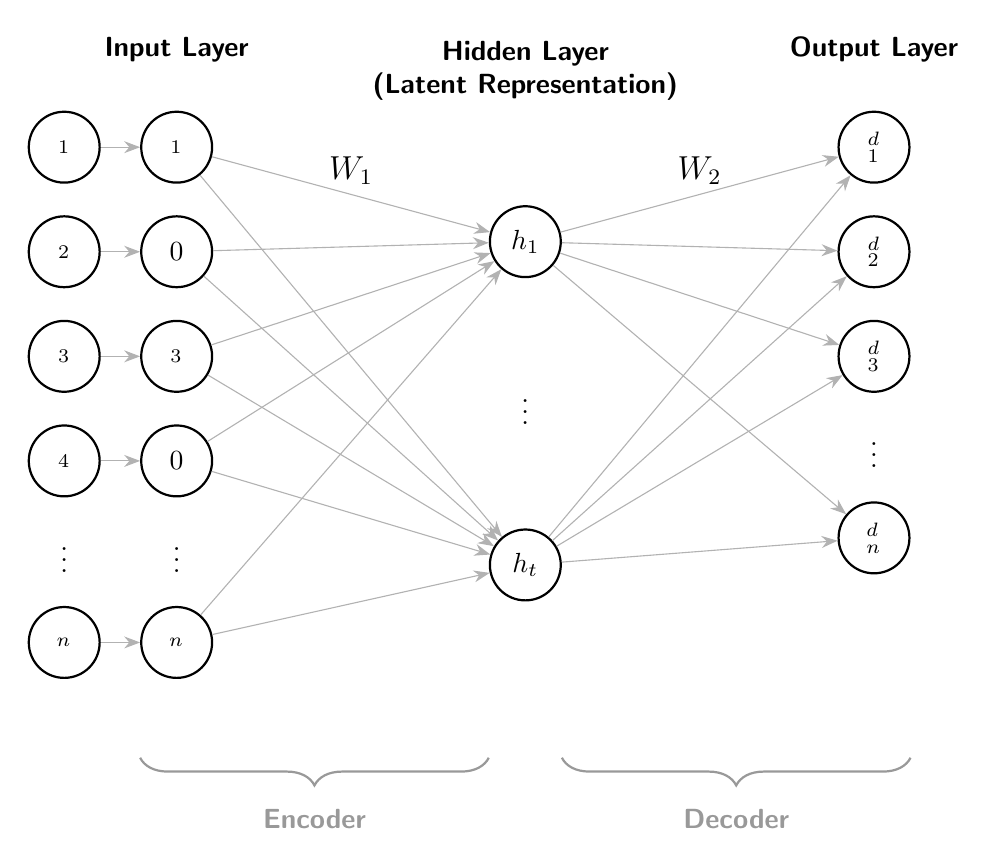
\begin{tikzpicture}[
    % Global Style Definitions
    node distance=1.2cm and 2.5cm,
    layer_node/.style={circle, draw=black, thick, minimum size=0.9cm, inner sep=0pt, fill=white, font=\sffamily},
    label_text/.style={font=\sffamily\bfseries, text centered},
    brace_style/.style={decorate, decoration={brace, amplitude=10pt, mirror}, thick, gray!80}
]

	
	\node[layer_node] (x10) {$\xbf_1$};
    \node[layer_node, below=0.4cm of x10] (x20) {$\xbf_2$};
    \node[layer_node, below=0.4cm of x20] (x30) {$\xbf_3$};
    \node[layer_node, below=0.4cm of x30] (x40) {$\xbf_4$};
    \node[below=0.3cm of x40] (xdots0) {$\vdots$};
    \node[layer_node, below=0.3cm of xdots0] (xn0) {$\xbf_n$};
    
    
    
    
    % --- 1. Draw Input Layer ---
    \node[layer_node, right=0.5cm of x10] (x1) {$\xbf_1$};
    \node[layer_node, below=0.4cm of x1] (x2) {$0$};
    \node[layer_node, below=0.4cm of x2] (x3) {$\xbf_3$};
    \node[layer_node, below=0.4cm of x3] (x4) {$0$};
    \node[below=0.3cm of x4] (xdots) {$\vdots$};
    \node[layer_node, below=0.3cm of xdots] (xn) {$\xbf_n$};
    
    \node[label_text, above=0.5cm of x1] {Input Layer};
    
    \draw[-{Stealth[scale=1.2]}, thin, gray!60] (x10) -- (x1);
    \draw[-{Stealth[scale=1.2]}, thin, gray!60] (x20) -- (x2);
    \draw[-{Stealth[scale=1.2]}, thin, gray!60] (x30) -- (x3);
    \draw[-{Stealth[scale=1.2]}, thin, gray!60] (x40) -- (x4);
    \draw[-{Stealth[scale=1.2]}, thin, gray!60] (xn0) -- (xn);

    % --- 2. Draw Hidden Layer (Code) ---
    % Centering the hidden layer relative to the input layer
    \coordinate (middle_input) at ($(x1.south)!0.5!(xn.north)$);
    \node[layer_node, right=3.5cm of x1, yshift=-1.2cm] (h1) {$h_1$};
    \node[below=1.2cm of h1] (hdots) {$\vdots$};
    \node[layer_node, below=1.2cm of hdots] (ht) {$h_t$};
    
    \node[label_text, above=1.2cm of h1, align=center] {Hidden Layer \\ (Latent Representation)};

    % --- 3. Draw Output Layer ---
    \node[layer_node, right=3.5cm of h1, yshift=1.2cm] (y1) {$\xbf_1^d$};
    \node[layer_node, below=0.4cm of y1] (y2) {$\xbf_2^d$};
    \node[layer_node, below=0.4cm of y2] (y3) {$\xbf_3^d$};
    \node[below=0.3cm of y3] (ydots) {$\vdots$};
    \node[layer_node, below=0.3cm of ydots] (yn) {$\xbf_n^d$};
    
    \node[label_text, above=0.5cm of y1] {Output Layer};

    % --- 4. Draw Connections (Weights) ---
    % Using a loop for cleaner code
    \foreach \i in {x1, x2, x3, x4, xn}
        \foreach \j in {h1, ht}
            \draw[-{Stealth[scale=1.2]}, thin, gray!60] (\i) -- (\j);
            
    \foreach \i in {h1, ht}
        \foreach \j in {y1, y2, y3, yn}
            \draw[-{Stealth[scale=1.2]}, thin, gray!60] (\i) -- (\j);

    % --- 5. Weight Labels ---
    % Placed manually for better visibility
    \node[font=\large\bfseries] at ($(x1)!0.5!(h1) + (0,0.3)$) {$W_1$};
    \node[font=\large\bfseries] at ($(h1)!0.5!(y1) + (0,0.3)$) {$W_2$};

    % --- 6. Braces (Encoder / Decoder) ---
    \draw[brace_style] ([yshift=-1cm]x1.west |- xn.south) -- ([yshift=-1cm]h1.west |- xn.south) 
        node[midway, below=15pt, font=\sffamily\bfseries] {Encoder};
        
    \draw[brace_style] ([yshift=-1cm]h1.east |- xn.south) -- ([yshift=-1cm]y1.east |- xn.south) 
        node[midway, below=15pt, font=\sffamily\bfseries] {Decoder};

\end{tikzpicture}
}
\footnotesize

\end{column}



\end{columns}


\end{frame}

\begin{frame}{Stacked AutoEncoder}



\end{frame}

\begin{frame}{Reading List}

\begin{enumerate}
\item Vincent, P., Larochelle, H., Bengio, Y., \& Manzagol, P. A. (2008, July). Extracting and composing robust features with denoising autoencoders. In Proceedings of the 25th international conference on Machine learning (pp. 1096-1103). \url{https://dl.acm.org/doi/pdf/10.1145/1390156.1390294}
\item Alain, Guillaume, and Yoshua Bengio. "What regularized auto-encoders learn from the data-generating distribution." The Journal of Machine Learning Research 15, no. 1 (2014): 3563-3593. \url{https://www.jmlr.org/papers/volume15/alain14a/alain14a.pdf}
\end{enumerate}

\end{frame}

    
\end{document}